\documentclass[]{article}
\usepackage{lmodern}
\usepackage{amssymb,amsmath}
\usepackage{ifxetex,ifluatex}
\usepackage{fixltx2e} % provides \textsubscript
\ifnum 0\ifxetex 1\fi\ifluatex 1\fi=0 % if pdftex
  \usepackage[T1]{fontenc}
  \usepackage[utf8]{inputenc}
\else % if luatex or xelatex
  \ifxetex
    \usepackage{mathspec}
  \else
    \usepackage{fontspec}
  \fi
  \defaultfontfeatures{Ligatures=TeX,Scale=MatchLowercase}
\fi
% use upquote if available, for straight quotes in verbatim environments
\IfFileExists{upquote.sty}{\usepackage{upquote}}{}
% use microtype if available
\IfFileExists{microtype.sty}{%
\usepackage{microtype}
\UseMicrotypeSet[protrusion]{basicmath} % disable protrusion for tt fonts
}{}
\usepackage[margin=1in]{geometry}
\usepackage{hyperref}
\hypersetup{unicode=true,
            pdftitle={DATA 606 - Homework 7},
            pdfauthor={Joshua Sturm},
            pdfborder={0 0 0},
            breaklinks=true}
\urlstyle{same}  % don't use monospace font for urls
\usepackage{color}
\usepackage{fancyvrb}
\newcommand{\VerbBar}{|}
\newcommand{\VERB}{\Verb[commandchars=\\\{\}]}
\DefineVerbatimEnvironment{Highlighting}{Verbatim}{commandchars=\\\{\}}
% Add ',fontsize=\small' for more characters per line
\usepackage{framed}
\definecolor{shadecolor}{RGB}{248,248,248}
\newenvironment{Shaded}{\begin{snugshade}}{\end{snugshade}}
\newcommand{\KeywordTok}[1]{\textcolor[rgb]{0.13,0.29,0.53}{\textbf{#1}}}
\newcommand{\DataTypeTok}[1]{\textcolor[rgb]{0.13,0.29,0.53}{#1}}
\newcommand{\DecValTok}[1]{\textcolor[rgb]{0.00,0.00,0.81}{#1}}
\newcommand{\BaseNTok}[1]{\textcolor[rgb]{0.00,0.00,0.81}{#1}}
\newcommand{\FloatTok}[1]{\textcolor[rgb]{0.00,0.00,0.81}{#1}}
\newcommand{\ConstantTok}[1]{\textcolor[rgb]{0.00,0.00,0.00}{#1}}
\newcommand{\CharTok}[1]{\textcolor[rgb]{0.31,0.60,0.02}{#1}}
\newcommand{\SpecialCharTok}[1]{\textcolor[rgb]{0.00,0.00,0.00}{#1}}
\newcommand{\StringTok}[1]{\textcolor[rgb]{0.31,0.60,0.02}{#1}}
\newcommand{\VerbatimStringTok}[1]{\textcolor[rgb]{0.31,0.60,0.02}{#1}}
\newcommand{\SpecialStringTok}[1]{\textcolor[rgb]{0.31,0.60,0.02}{#1}}
\newcommand{\ImportTok}[1]{#1}
\newcommand{\CommentTok}[1]{\textcolor[rgb]{0.56,0.35,0.01}{\textit{#1}}}
\newcommand{\DocumentationTok}[1]{\textcolor[rgb]{0.56,0.35,0.01}{\textbf{\textit{#1}}}}
\newcommand{\AnnotationTok}[1]{\textcolor[rgb]{0.56,0.35,0.01}{\textbf{\textit{#1}}}}
\newcommand{\CommentVarTok}[1]{\textcolor[rgb]{0.56,0.35,0.01}{\textbf{\textit{#1}}}}
\newcommand{\OtherTok}[1]{\textcolor[rgb]{0.56,0.35,0.01}{#1}}
\newcommand{\FunctionTok}[1]{\textcolor[rgb]{0.00,0.00,0.00}{#1}}
\newcommand{\VariableTok}[1]{\textcolor[rgb]{0.00,0.00,0.00}{#1}}
\newcommand{\ControlFlowTok}[1]{\textcolor[rgb]{0.13,0.29,0.53}{\textbf{#1}}}
\newcommand{\OperatorTok}[1]{\textcolor[rgb]{0.81,0.36,0.00}{\textbf{#1}}}
\newcommand{\BuiltInTok}[1]{#1}
\newcommand{\ExtensionTok}[1]{#1}
\newcommand{\PreprocessorTok}[1]{\textcolor[rgb]{0.56,0.35,0.01}{\textit{#1}}}
\newcommand{\AttributeTok}[1]{\textcolor[rgb]{0.77,0.63,0.00}{#1}}
\newcommand{\RegionMarkerTok}[1]{#1}
\newcommand{\InformationTok}[1]{\textcolor[rgb]{0.56,0.35,0.01}{\textbf{\textit{#1}}}}
\newcommand{\WarningTok}[1]{\textcolor[rgb]{0.56,0.35,0.01}{\textbf{\textit{#1}}}}
\newcommand{\AlertTok}[1]{\textcolor[rgb]{0.94,0.16,0.16}{#1}}
\newcommand{\ErrorTok}[1]{\textcolor[rgb]{0.64,0.00,0.00}{\textbf{#1}}}
\newcommand{\NormalTok}[1]{#1}
\usepackage{graphicx,grffile}
\makeatletter
\def\maxwidth{\ifdim\Gin@nat@width>\linewidth\linewidth\else\Gin@nat@width\fi}
\def\maxheight{\ifdim\Gin@nat@height>\textheight\textheight\else\Gin@nat@height\fi}
\makeatother
% Scale images if necessary, so that they will not overflow the page
% margins by default, and it is still possible to overwrite the defaults
% using explicit options in \includegraphics[width, height, ...]{}
\setkeys{Gin}{width=\maxwidth,height=\maxheight,keepaspectratio}
\IfFileExists{parskip.sty}{%
\usepackage{parskip}
}{% else
\setlength{\parindent}{0pt}
\setlength{\parskip}{6pt plus 2pt minus 1pt}
}
\setlength{\emergencystretch}{3em}  % prevent overfull lines
\providecommand{\tightlist}{%
  \setlength{\itemsep}{0pt}\setlength{\parskip}{0pt}}
\setcounter{secnumdepth}{0}
% Redefines (sub)paragraphs to behave more like sections
\ifx\paragraph\undefined\else
\let\oldparagraph\paragraph
\renewcommand{\paragraph}[1]{\oldparagraph{#1}\mbox{}}
\fi
\ifx\subparagraph\undefined\else
\let\oldsubparagraph\subparagraph
\renewcommand{\subparagraph}[1]{\oldsubparagraph{#1}\mbox{}}
\fi

%%% Use protect on footnotes to avoid problems with footnotes in titles
\let\rmarkdownfootnote\footnote%
\def\footnote{\protect\rmarkdownfootnote}

%%% Change title format to be more compact
\usepackage{titling}

% Create subtitle command for use in maketitle
\newcommand{\subtitle}[1]{
  \posttitle{
    \begin{center}\large#1\end{center}
    }
}

\setlength{\droptitle}{-2em}
  \title{DATA 606 - Homework 7}
  \pretitle{\vspace{\droptitle}\centering\huge}
  \posttitle{\par}
  \author{Joshua Sturm}
  \preauthor{\centering\large\emph}
  \postauthor{\par}
  \predate{\centering\large\emph}
  \postdate{\par}
  \date{11/12/2017}


\begin{document}
\maketitle

\subsection{7.24 Nutrition at Starbucks, Part
1.}\label{nutrition-at-starbucks-part-1.}

The scatterplot below shows the relationship between the number of
calories and amount of carbohydrates (in grams) Starbucks food menu
items contain. Since Starbucks only lists the number of calories on the
display items, we are interested in predicting the amount of carbs a
menu item has based on its calorie content. 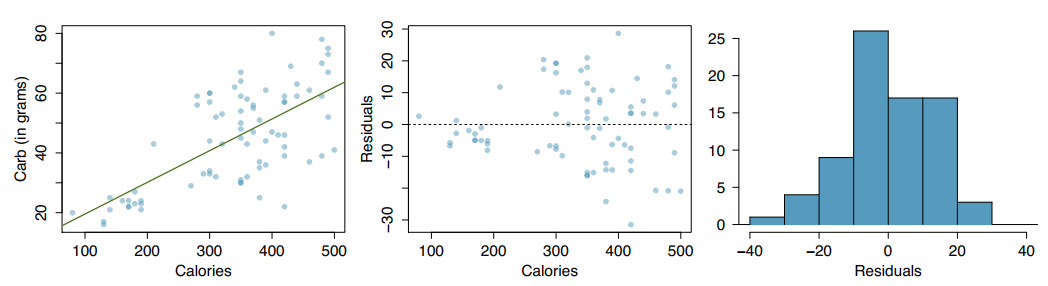
\includegraphics{7.24.PNG}
(a) Describe the relationship between number of calories and amount of
carbohydrates (in grams) that Starbucks food menu items contain.\\
(b) In this scenario, what are the explanatory and response variables?\\
(c) Why might we want to fit a regression line to these data?\\
(d) Do these data meet the conditions required for fitting a least
squares line?

\subsubsection{(a) Solution}\label{a-solution}

There is a small, positive correlation between number of calories and
amount of carbs.

\subsubsection{(b) Solution}\label{b-solution}

The explanatory variable is the number of calories, and the response
variable is the amount of carbohydrates.

\subsubsection{(c) Solution}\label{c-solution}

We can fit a regression line to predict the amount of carbs a food item
will have based on the number of calories.

\subsubsection{(d) Solution}\label{d-solution}

From section 7.7.2, there are four conditions for fitting a least
squares line: Linearity, Nearly normal residuals, Constant variability,
and Independent observations. There is a small linear relationship. The
histogram of residuals is close enough to be nearly normal. Constant
variability may be the biggest issue; the residuals in the middle plot
are not really clustered around the middle line.

\subsection{7.26 Body measurements, Part
III.}\label{body-measurements-part-iii.}

Exercise 7.15 introduces data on shoulder girth and height of a group of
individuals. The mean shoulder girth is 107.20 cm with a standard
deviation of 10.37 cm. The mean height is 171.14 cm with a standard
deviation of 9.41 cm. The correlation between height and shoulder girth
is 0.67.

\begin{enumerate}
\def\labelenumi{(\alph{enumi})}
\tightlist
\item
  Write the equation of the regression line for predicting height.\\
\item
  Interpret the slope and the intercept in this context.\\
\item
  Calculate \(R^2\) of the regression line for predicting height from
  shoulder girth, and interpret it in the context of the application.\\
\item
  A randomly selected student from your class has a shoulder girth of
  100 cm. Predict the height of this student using the model.\\
\item
  The student from part (d) is 160 cm tall. Calculate the residual, and
  explain what this residual means.\\
\item
  A one year old has a shoulder girth of 56 cm. Would it be appropriate
  to use this linear model to predict the height of this child?
\end{enumerate}

\subsubsection{(a) Solution}\label{a-solution-1}

The formula for the regression line is:
\(y = \beta_0 +\beta_1 \times x\).\\
From equation 7.12, \(b_1 = \frac{s_y}{s_x}R\).\\
From equation 7.15, \(y - y_0 = b_1(x - x_0)\).\\
\(x_0 = 107.2, \quad y_0 = 171.14\).\\
\(s_x = 10.37, \quad s_y = 9.41\).\\
\(R = 0.67\).

\begin{Shaded}
\begin{Highlighting}[]
\NormalTok{x0 <-}\StringTok{ }\FloatTok{107.2}
\NormalTok{y0 <-}\StringTok{ }\FloatTok{171.14}

\NormalTok{sx <-}\StringTok{ }\FloatTok{10.37}
\NormalTok{sy <-}\StringTok{ }\FloatTok{9.41}
\NormalTok{r <-}\StringTok{ }\FloatTok{0.67}

\NormalTok{b1 <-}\StringTok{ }\NormalTok{(sy }\OperatorTok{/}\StringTok{ }\NormalTok{sx) }\OperatorTok{*}\StringTok{ }\NormalTok{r}

\NormalTok{b0 <-}\StringTok{ }\NormalTok{y0 }\OperatorTok{-}\StringTok{ }\NormalTok{(b1 }\OperatorTok{*}\StringTok{ }\NormalTok{x0)}
\end{Highlighting}
\end{Shaded}

\(y = 105.9650878 + 0.6079749\times x\).

\subsubsection{(b) Solution}\label{b-solution-1}

\(\widehat{height} = 105.9650878 + 0.6079749\times \text{shoulder girth}\).\\
The slope tells us that each centimeter of shoulder girth increases
height by 0.61 centimeters.\\
The intercept tells us that a (hypothetical) shoulder girth of 0 would
mean a height of \(\approx 106\) centimeters.

\subsubsection{(c) Solution}\label{c-solution-1}

\(R^2 = (0.67)^2 = 0.4489\).\\
44.89\% of the variation in height can be explained by our model.

\subsubsection{(d) Solution}\label{d-solution-1}

Using the equation from part (a):
\(\widehat{height} = 105.9650878 + 0.6079749 \times 100 = 166.7625805\).

\subsubsection{(e) Solution}\label{e-solution}

Equation for residuals: \(e_i = y_i - \hat{y}_i\).\\
\(e_i = 160 - 166.7625805 = -6.762581\).\\
A negative value tells us that our model overestimated the actual
height.

\subsubsection{(f) Solution}\label{f-solution}

Our model only covers shoulder girth in the range of 85-135 cm. A value
of 56 is way outside our range, so it would not be appropriate to use
our model to predict the height of this child.

\subsection{7.30 Cats, Part I.}\label{cats-part-i.}

The following regression output is for predicting the heart weight (in
g) of cats from their body weight (in kg). The coeffcients are estimated
using a dataset of 144 domestic cats.

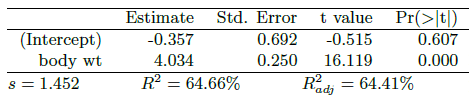
\includegraphics{7.30a.PNG} 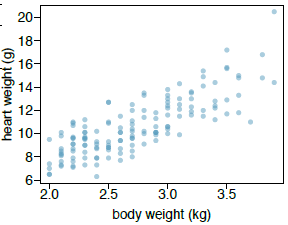
\includegraphics{7.30b.PNG}

\begin{enumerate}
\def\labelenumi{(\alph{enumi})}
\tightlist
\item
  Write out the linear model.\\
\item
  Interpret the intercept.\\
\item
  Interpret the slope.\\
\item
  Interpret \(R^2\).\\
\item
  Calculate the correlation coeffcient.
\end{enumerate}

\subsubsection{(a) Solution}\label{a-solution-2}

\(\widehat{heart \ weight} = -0.357 + 4.034 \times \text{body weight}\).

\subsubsection{(b) Solution}\label{b-solution-2}

If a cat weighed 0 kg, they'd have a heart weight of -0.357.

\subsubsection{(c) Solution}\label{c-solution-2}

For every kilogram of body weight, the heart weight increases by just
over 4 times.

\subsubsection{(d) Solution}\label{d-solution-2}

\(R^2\) tells us that 64.66\% of the variability in heart weight can be
explained by our linear model.

\subsubsection{(e) Solution}\label{e-solution-1}

The correlation coefficient is given by \(R\).\\
\(\sqrt{R} = \sqrt{0.6466} = 0.8041144\).

\subsection{7.40 Rate my professor.}\label{rate-my-professor.}

Many college courses conclude by giving students the opportunity to
evaluate the course and the instructor anonymously. However, the use of
these student evaluations as an indicator of course quality and teaching
effectiveness is often criticized because these measures may reflect the
influence of non-teaching related characteristics, such as the physical
appearance of the instructor. Researchers at University of Texas, Austin
collected data on teaching evaluation score (higher score means better)
and standardized beauty score (a score of 0 means average, negative
score means below average, and a positive score means above average) for
a sample of 463 professors.24 The scatterplot below shows the
relationship between these variables, and also provided is a regression
output for predicting teaching evaluation score from beauty score.

\begin{figure}
\centering
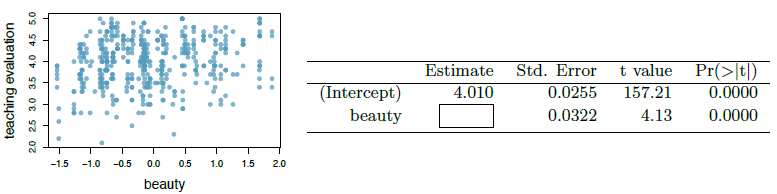
\includegraphics{7.40a.PNG}
\caption{}
\end{figure}

\begin{enumerate}
\def\labelenumi{(\alph{enumi})}
\tightlist
\item
  Given that the average standardized beauty score is -0.0883 and
  average teaching evaluation score is 3.9983, calculate the slope.
  Alternatively, the slope may be computed using just the information
  provided in the model summary table.\\
\item
  Do these data provide convincing evidence that the slope of the
  relationship between teaching evaluation and beauty is positive?
  Explain your reasoning.\\
\item
  List the conditions required for linear regression and check if each
  one is satisfied for this model based on the following diagnostic
  plots
\end{enumerate}

\begin{figure}
\centering
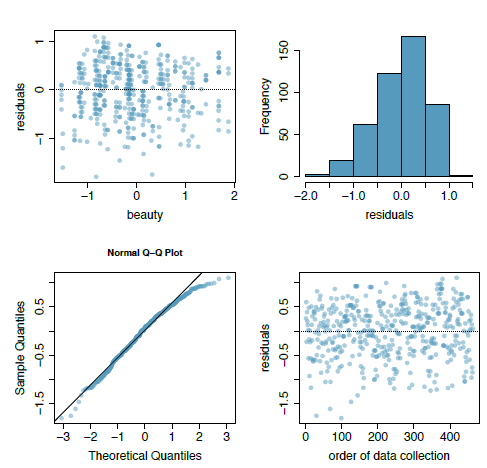
\includegraphics{7.40b.PNG}
\caption{}
\end{figure}

\subsubsection{(a) Solution}\label{a-solution-3}

\(y = \beta_0 +\beta_1 \times x \quad \to \quad 3.9983 = 4.010 + \beta_1 \times -0.0883\).\\
\(\beta_1 = \frac{3.9983 - 4.010}{-0.0883} \quad \to \quad \beta_1 = 0.1325028\).

\subsubsection{(b) Solution}\label{b-solution-3}

Yes, the slope is positive, so there is a positive relationship.
Furthermore, we could set up a hypothesis test and find the p-value,
which would be nearly 0.

\subsubsection{(c) Solution}\label{c-solution-3}

As mentioned in the first problem, there are four conditions for fitting
a least squares line: Linearity, Nearly normal residuals, Constant
variability, and Independent observations. There may be a slight linear
relationship, as seen in the scatterplot. From the histogram and Q-Q
plot, we can see that the residuals are nearly normal. The scatterplot
does have constant variability. Lastly, independence can be assumed.
Since all the conditions have been satisfied, the model is a good fit.


\end{document}
